\documentclass[12pt,a4paper]{article}
\usepackage[utf8]{inputenc}
\usepackage[T1]{fontenc}
\usepackage[polish]{babel}
\usepackage{geometry}
\usepackage{graphicx}
\usepackage{booktabs}
\usepackage{caption}
\usepackage{subcaption}
\usepackage{amsmath}
\usepackage{hyperref}
\usepackage{float}
\usepackage{array}
\usepackage{xcolor}
\usepackage{parskip}

\geometry{margin=2.5cm}

\hypersetup{
    urlcolor=blue
}

\title{
    \textbf{Pr3: Implementacja i analiza efektywności algorytmów} \\
    \textbf{wyznaczania najkrótszej ścieżki w grafie} \\
    \large Dijkstra i Bellman-Ford oraz wpływ struktur danych na efektywność
}
\author{Joachim Szewior 263943}
\date{Maj 2026}

\begin{document}

\maketitle
\tableofcontents
\newpage

% =========================================================
\section{Cel i zakres zadania}

Celem zadania projektowego Pr3 była implementacja oraz analiza porównawcza dwóch algorytmów wyznaczania najkrótszej ścieżki w grafie:

\begin{itemize}
    \item \textbf{algorytmu Dijkstry} wyznaczającego najkrótszą ścieżkę w grafach z nieujemnymi wagami krawędzi, z wykorzystaniem kopca jako priorytetowej kolejki do wyboru wierzchołków o najmniejszym koszcie,
    \item \textbf{algorytmu Bellmana-Forda} będącego algorytmem ogólnym, działającym na grafach z dowolnymi wagami krawędzi (w tym ujemnymi), zdolnym do wykrywania cykli o ujemnej wadze.
\end{itemize}

W ramach zadania zrealizowano trzy główne punkty:
\begin{enumerate}
    \item implementację obu algorytmów dla trzech różnych struktur danych,
    \item testowanie algorytmów na grafach o różnych rozmiarach i gęstościach,
    \item porównanie efektywności algorytmów przy różnych strukturach danych.
\end{enumerate}

Eksperymenty przeprowadzono dla trzech reprezentacji grafu:
\begin{enumerate}
    \item \textbf{Macierz wag} będąca macierzą $V \times V$ przechowującą wagi krawędzi,
    \item \textbf{Lista krawędzi} będąca listą wszystkich krawędzi w postaci trójek $(u, v, w)$,
    \item \textbf{Lista sąsiedztwa} przechowująca dla każdego wierzchołka listę jego sąsiadów wraz z wagami krawędzi.
\end{enumerate}

Zbadano wpływ rozmiaru grafu ($V \in \{50, 100, 250, 500, 1000\}$) oraz jego gęstości ($d \in \{0{,}1;\; 0{,}3;\; 0{,}6;\; 0{,}9\}$) na czas wykonania, zużycie pamięci i liczbę operacji relaksacji.

% =========================================================
\section{Opis algorytmów i szczegóły implementacji}

\subsection{Algorytm Dijkstry}

Algorytm Dijkstry wyznacza najkrótsze ścieżki z jednego źródła do wszystkich pozostałych wierzchołków w grafie z nieujemnymi wagami. Działa w sposób zachłanny: w każdym kroku wybiera wierzchołek o najmniejszej aktualnie znalezionej odległości i relaksuje jego krawędzie wychodzące.

Złożoność czasowa wynosi $O((V + E) \log V)$ przy użyciu kopca binarnego.

\subsubsection*{Szczegóły implementacji}

W implementacji zastosowano kopiec binarny (\texttt{heapq}) z techniką leniwego usuwania. Wierzchołek wyciągnięty z kopca jest pomijany jeśli był już odwiedzony. Zbiór \texttt{visited} zapobiega wielokrotnemu przetwarzaniu tego samego wierzchołka. Jako operację zliczaną przyjęto każde sprawdzenie sąsiada wierzchołka $u$, co odpowiada liczbie krawędzi wychodzących z odwiedzonych wierzchołków.

\subsection{Algorytm Bellmana-Forda}

Algorytm Bellmana-Forda obsługuje krawędzie o ujemnych wagach i wykrywa ujemne cykle. Wykonuje co najwyżej $V - 1$ rund relaksacji wszystkich krawędzi, a następnie dodatkową rundę sprawdzającą obecność ujemnego cyklu. Złożoność czasowa wynosi $O(V \cdot E)$.

\subsubsection*{Szczegóły implementacji}

Zastosowano optymalizację wczesnego zakończenia: jeśli w danej iteracji żadna odległość nie uległa poprawie (flaga \texttt{updated = False}), algorytm kończy pracę przed wykonaniem wszystkich $V-1$ rund. Na grafach bez ujemnych wag rzeczywista liczba iteracji jest dzięki temu często mniejsza niż teoretyczne maksimum. Jako operację zliczaną przyjęto każde sprawdzenie krawędzi, wliczając w to dodatkową rundę wykrywania cyklu.

% =========================================================
\section{Metodologia}

\subsection{Parametry eksperymentów}

Testy przeprowadzono dla losowo generowanych grafów skierowanych z wagami całkowitymi. Wierzchołkiem źródłowym był zawsze wierzchołek o numerze $0$. Zakresy wag różniły się w zależności od algorytmu:

\begin{itemize}
    \item Dijkstra: wagi krawędzi z zakresu $[1, 100]$ (wyłącznie dodatnie),
    \item Bellman-Ford: wagi krawędzi z zakresu $[-20, 100]$ (możliwe ujemne).
\end{itemize}

Każda kombinacja parametrów była powtarzana 5 razy z różnymi ziarnami generatora losowego, a wyniki uśredniano. Zbierano następujące metryki:
\begin{itemize}
    \item średni czas wykonania wraz z odchyleniem standardowym [ms],
    \item zużycie pamięci przez strukturę grafu [B],
    \item liczbę operacji relaksacji krawędzi.
\end{itemize}

\subsection{Pomiar pamięci}

Zużycie pamięci mierzono analitycznie. Każda klasa struktury grafu implementuje metodę memory\_bytes() która szacuje rozmiar.

\subsection{Test wykrywania ujemnych cykli}

Dla każdej struktury danych wygenerowano dodatkowy graf o $V = 20$ wierzchołkach i gęstości $d = 0{,}3$. Do tego grafu ręcznie dodano ujemny cykl złożony z krawędzi $0 \to 1$, $1 \to 2$ oraz $2 \to 0$, każda z wagą $-10$. Cykl ten gwarantuje obecność ujemnego cyklu osiągalnego ze źródła.

\subsection{Środowisko testowe}

Eksperymenty wykonano w języku Python 3.12. Pomiar czasu opierał się na funkcji \texttt{time.perf\_counter()} zapewniającej wysoką rozdzielczość pomiaru.

% =========================================================
\section{Wyniki eksperymentów}

\subsection{Czas wykonania a rozmiar grafu}

\begin{figure}[H]
    \centering
    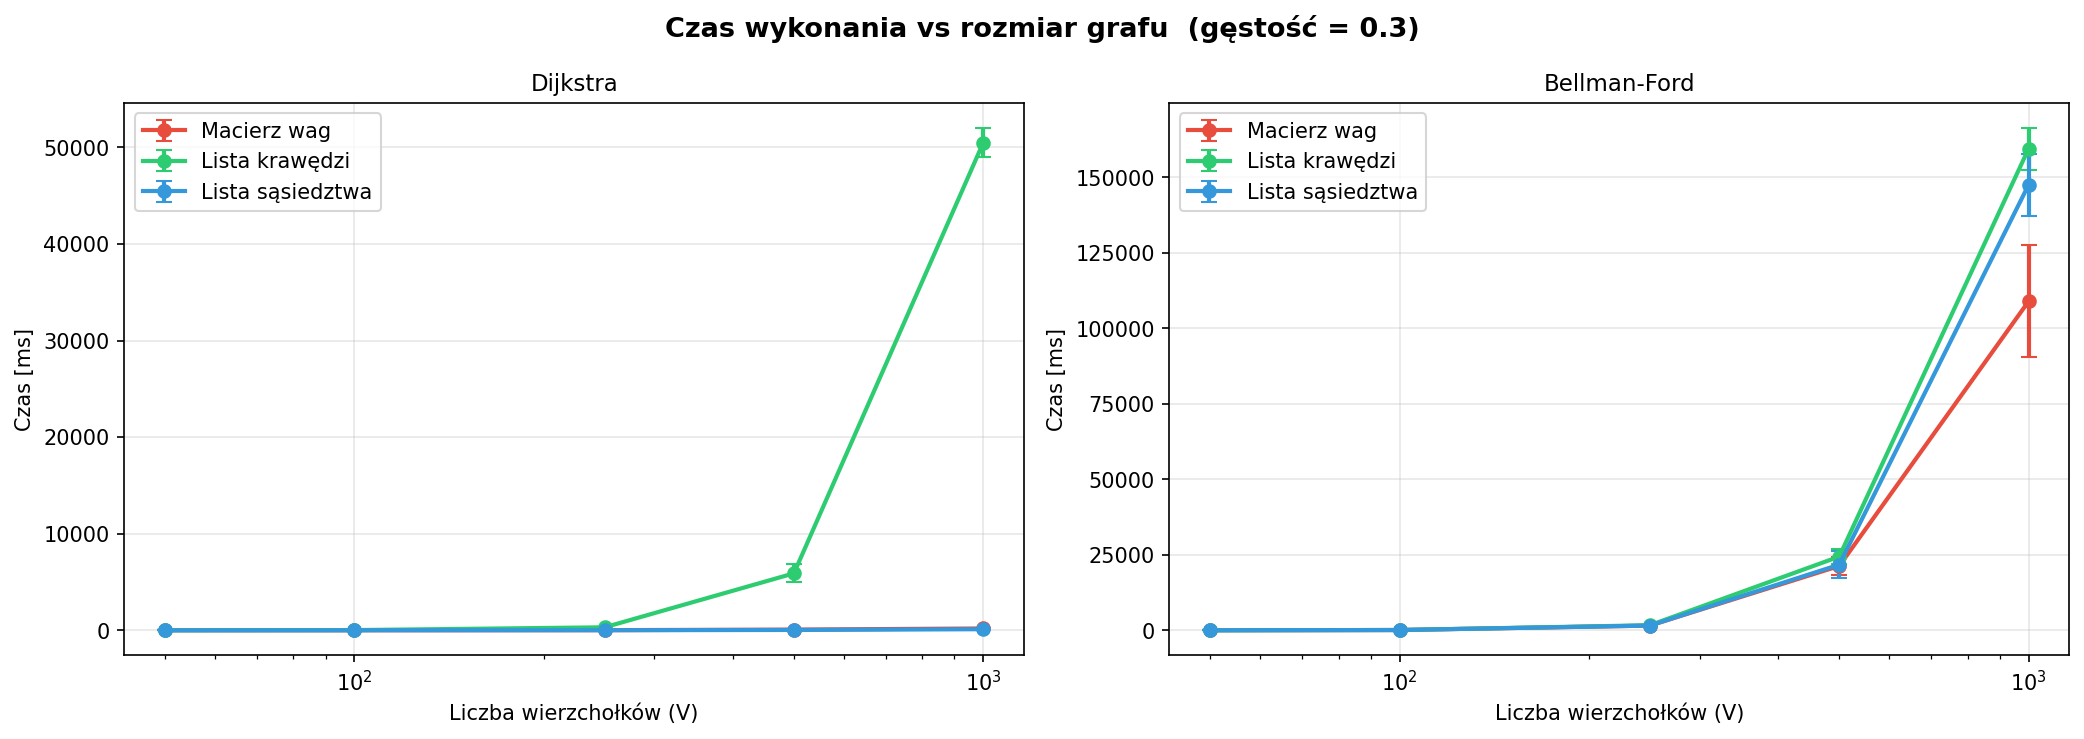
\includegraphics[width=\textwidth]{results/time_vs_size.png}
    \caption{Czas wykonania algorytmów Dijkstry i Bellmana-Forda w zależności od liczby wierzchołków ($d = 0{,}3$) dla trzech reprezentacji grafu.}
    \label{fig:time_vs_size}
\end{figure}

Na rysunku~\ref{fig:time_vs_size} można zaobserwować kilka istotnych zależności:
\begin{itemize}
    \item Lista sąsiedztwa oraz Macierz wag są o wiele szybsze niż lista krawędzi.
    \item Macierz wag okazała się być najszybsza dla algorytmu Bellmana-Forda.
    \item Bellman-Ford jest znacznie wolniejszy od Dijkstry. Dla $V = 1000$ różnica sięga trzech rzędów wielkości.
    \item Czas wykonania rośnie zgodnie z oczekiwaną złożonością teoretyczną obu algorytmów.
\end{itemize}

\subsection{Czas wykonania a gęstość grafu}

\begin{figure}[H]
    \centering
    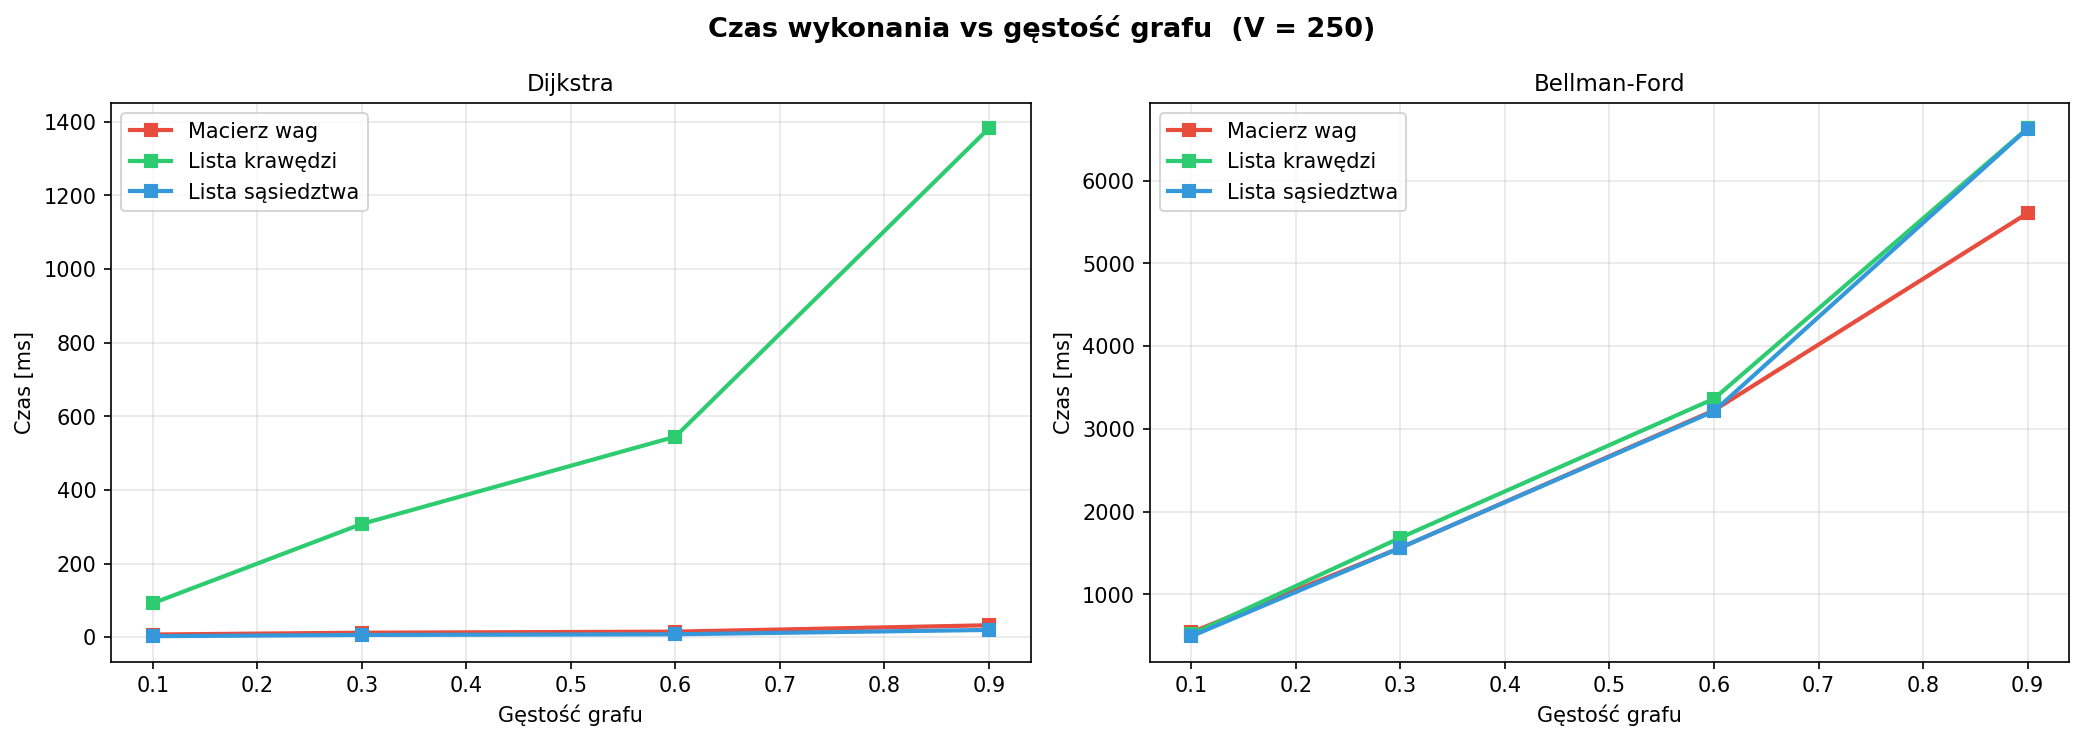
\includegraphics[width=\textwidth]{results/time_vs_density.png}
    \caption{Czas wykonania w zależności od gęstości grafu ($V = 250$).}
    \label{fig:time_vs_density}
\end{figure}

Rysunek~\ref{fig:time_vs_density} przedstawia wpływ gęstości grafu na czas wykonania dla $V = 250$:
\begin{itemize}
    \item Dla Dijkstry czas rośnie liniowo względem liczby krawędzi. Lista krawędzi wykazuje najsilniejszą zależność od gęstości. Przy $d = 0{,}9$ osiąga ona około 1382~ms.
    \item Dla Bellmana-Forda wszystkie trzy struktury skalują się podobnie, gdyż algorytm iteruje po wszystkich krawędziach $V-1$ razy niezależnie od użytej reprezentacji.
    \item Macierz wag i lista sąsiedztwa dla Dijkstry pozostają praktycznie nierozróżnialne w tej skali.
\end{itemize}

\subsection{Bezpośrednie porównanie obu algorytmów}

\begin{figure}[H]
    \centering
    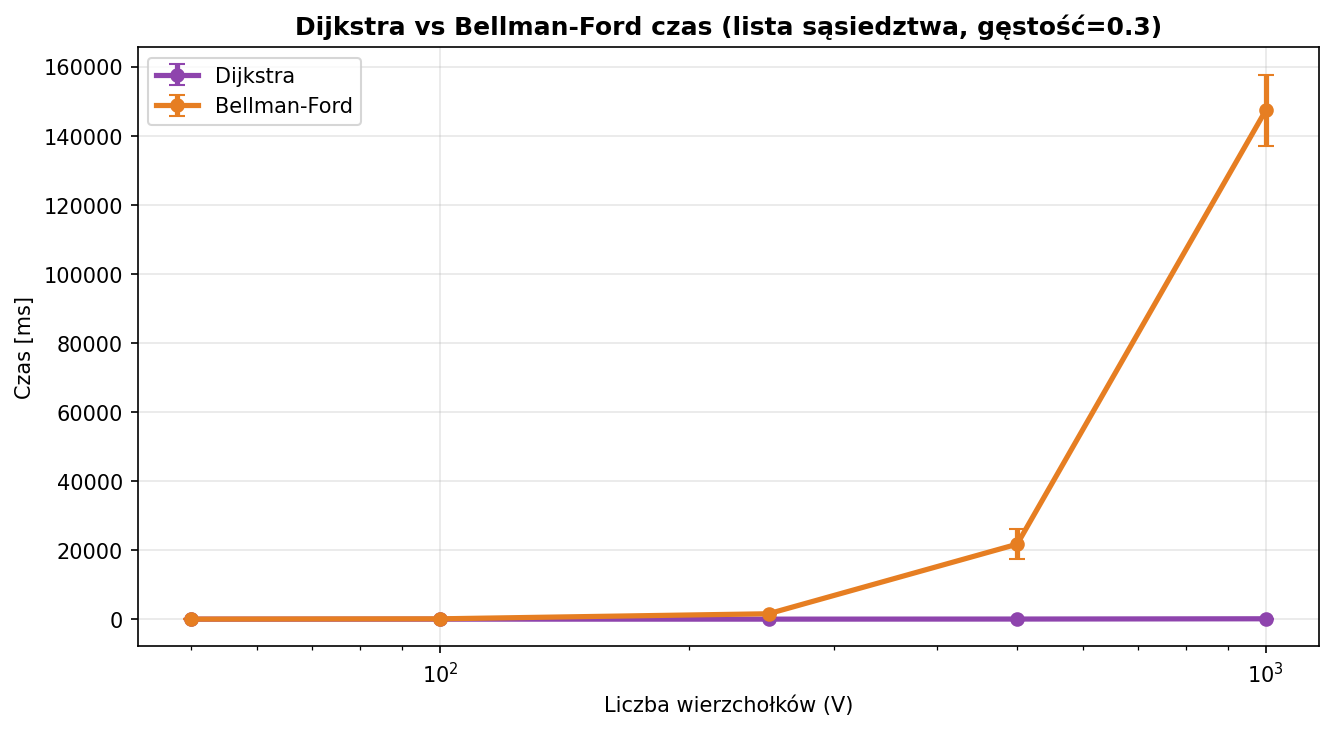
\includegraphics[width=0.85\textwidth]{results/dijkstra_vs_bellmanford.png}
    \caption{Porównanie czasu wykonania Dijkstry i Bellmana-Forda (lista sąsiedztwa, $d = 0{,}3$).}
    \label{fig:dijkstra_vs_bf}
\end{figure}

Rysunek~\ref{fig:dijkstra_vs_bf} bezpośrednio zestawia oba algorytmy dla listy sąsiedztwa. Dijkstra jest na tyle szybsza, że linia jej czasu praktycznie przylega do osi $x$ w porównaniu z Bellmanem-Fordem. Dla $V = 1000$ i $d = 0{,}3$:
\begin{itemize}
    \item Dijkstra (lista sąsiedztwa): $\approx 111$~ms,
    \item Bellman-Ford (lista sąsiedztwa): $\approx 147\,438$~ms.
\end{itemize}
Oznacza to przewagę Dijkstry o czynnik ponad \textbf{1300}.

\subsection{Zużycie pamięci}

\begin{figure}[H]
    \centering
    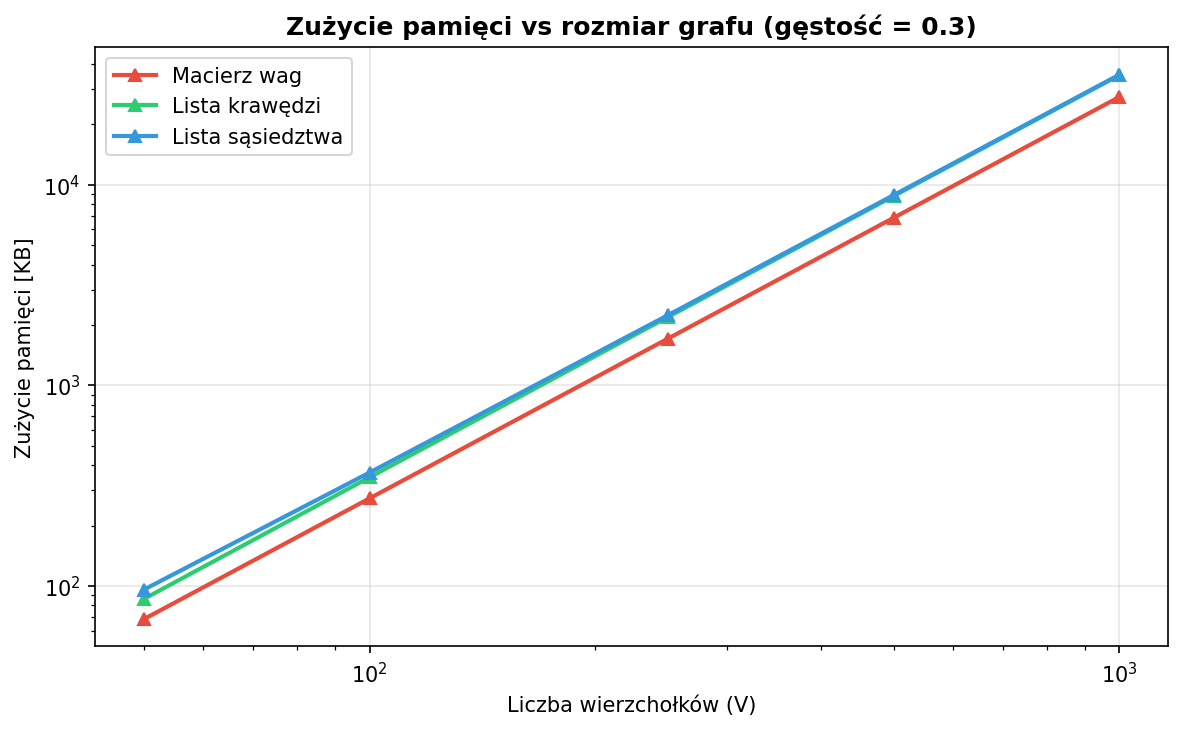
\includegraphics[width=0.85\textwidth]{results/memory_vs_size.png}
    \caption{Zużycie pamięci przez strukturę grafu w zależności od liczby wierzchołków ($d = 0{,}3$, skala logarytmiczna).}
    \label{fig:memory}
\end{figure}

Z rysunku~\ref{fig:memory} wynikają następujące obserwacje:
\begin{itemize}
    \item Macierz wag zużywa najmniej pamięci dla małych grafów.
    \item Lista krawędzi i lista sąsiedztwa mają praktycznie tę samą funkcję wzrostu pamięci i leżą prawie równolegle co macierz wag.
\end{itemize}

\subsection{Liczba operacji relaksacji}

\begin{figure}[H]
    \centering
    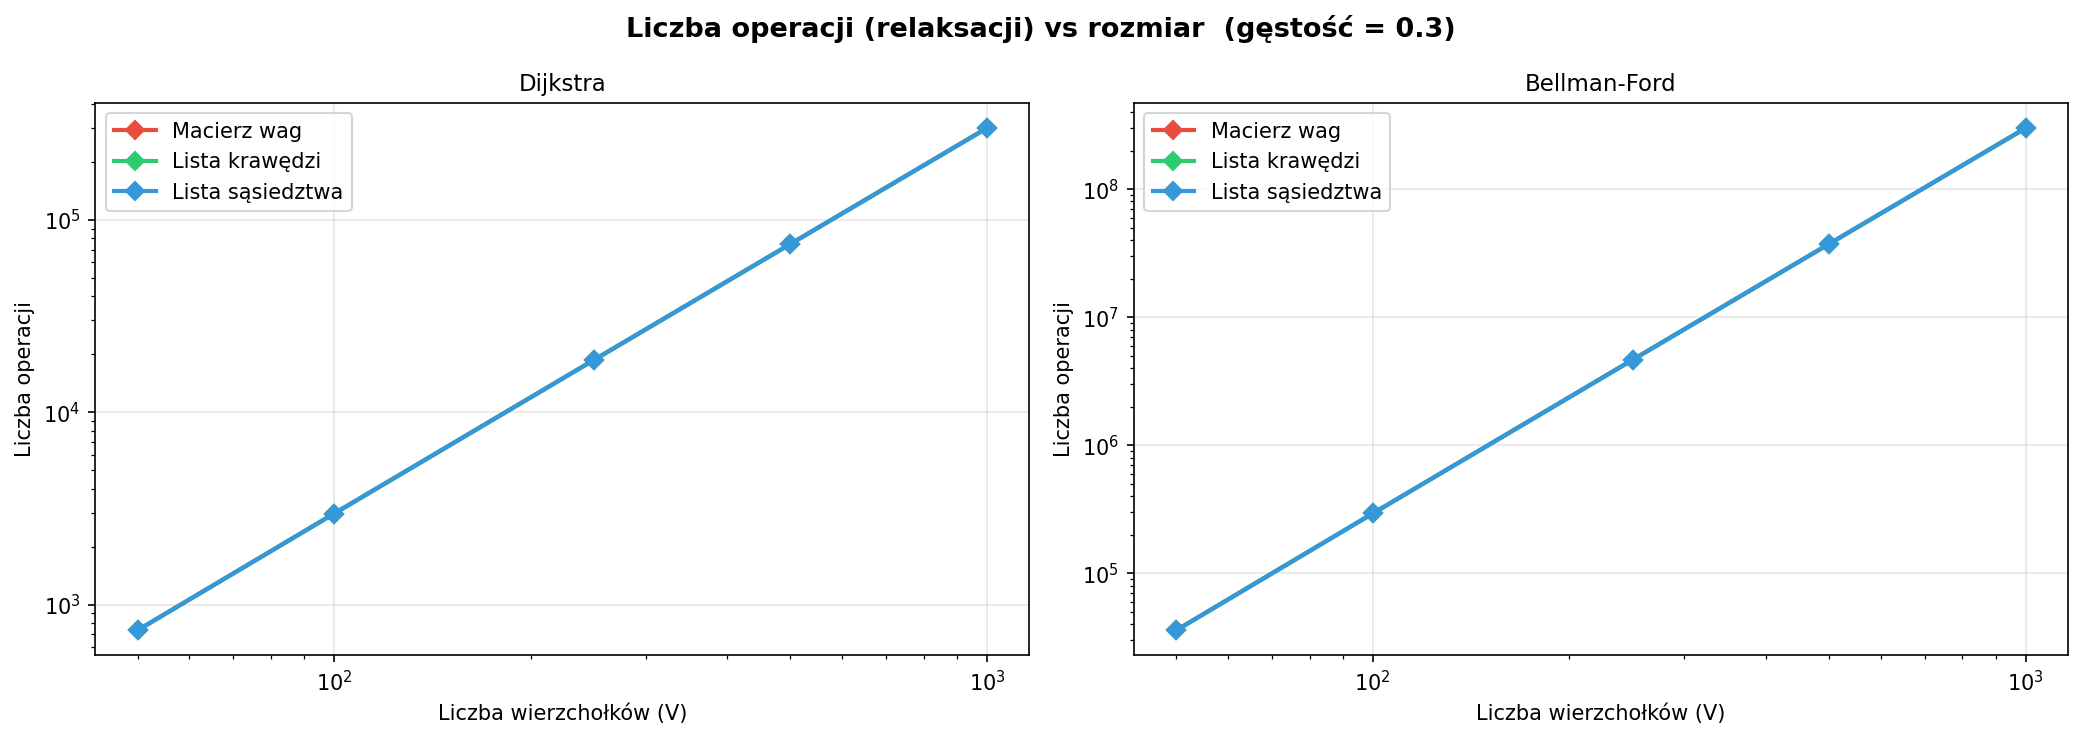
\includegraphics[width=\textwidth]{results/operations_vs_size.png}
    \caption{Liczba operacji relaksacji w zależności od rozmiaru grafu ($d = 0{,}3$, skala logarytmiczna).}
    \label{fig:operations}
\end{figure}

Rysunek~\ref{fig:operations} potwierdza teoretyczną złożoność obliczeniową obu algorytmów:
\begin{itemize}
    \item Dijkstra wykonuje liczbę operacji bliską liczbie krawędzi $E$, ponieważ każda krawędź jest sprawdzana co najwyżej raz.
    \item Ze względu na specyfikę algorytmu Bellmana-Forda potrzebuje on o wiele więcej operacji. Dla $V = 1000$ i $d = 0{,}3$ wynosi to około $299\,400\,306$ operacji, czyli ponad 1000 razy więcej niż dla Dijkstry.
    \item Liczba operacji jest niezależna od użytej reprezentacji grafu. Wszystkie trzy struktury przetwarzają ten sam zestaw krawędzi, co widać jako pokrywające się linie na wykresie.
\end{itemize}

% =========================================================
\section{Zestawienie wynikowe}

Tabele~\ref{tab:results_dijkstra} oraz~\ref{tab:results_bf} przedstawiają szczegółowe wyniki dla gęstości $d = 0{,}3$.

\begin{table}[H]
\centering
\caption{Wyniki algorytmu Dijkstry ($d = 0{,}3$)}
\label{tab:results_dijkstra}
\small
\begin{tabular}{rrrrrr}
\toprule
$V$ & Struktura & Czas [ms] & Odch.\ std.\ [ms] & Pamięć [KB] & Operacje \\
\midrule
50  & Macierz wag      & 0{,}820  & 0{,}081 & 68{,}4   & 735 \\
50  & Lista krawędzi   & 2{,}995  & 0{,}078 & 86{,}2   & 735 \\
50  & Lista sąsiedztwa & 0{,}441  & 0{,}019 & 95{,}9   & 735 \\
\midrule
100 & Macierz wag      & 2{,}182  & 0{,}078 & 273{,}4  & 2\,970 \\
100 & Lista krawędzi   & 18{,}417 & 0{,}623 & 348{,}1  & 2\,970 \\
100 & Lista sąsiedztwa & 1{,}259  & 0{,}088 & 367{,}6  & 2\,970 \\
\midrule
250 & Macierz wag      & 12{,}277 & 0{,}111 & 1\,709{,}0 & 18\,675 \\
250 & Lista krawędzi   & 307{,}648 & 14{,}324 & 2\,188{,}5 & 18\,675 \\
250 & Lista sąsiedztwa & 6{,}180  & 0{,}130 & 2\,237{,}3 & 18\,675 \\
\midrule
500 & Macierz wag      & 70{,}563 & 0{,}727  & 6\,835{,}9  & 74\,850 \\
500 & Lista krawędzi   & 5\,895{,}133 & 927{,}132 & 8\,771{,}5 & 74\,850 \\
500 & Lista sąsiedztwa & 32{,}868 & 1{,}288  & 8\,869{,}1  & 74\,850 \\
\midrule
1000 & Macierz wag     & 185{,}753 & 60{,}266  & 27\,343{,}8 & 299\,700 \\
1000 & Lista krawędzi  & 50\,486{,}154 & 1\,521{,}980 & 35\,121{,}1 & 299\,700 \\
1000 & Lista sąsiedztwa & 110{,}838 & 3{,}565 & 35\,316{,}4 & 299\,700 \\
\bottomrule
\end{tabular}
\end{table}

\begin{table}[H]
\centering
\caption{Wyniki algorytmu Bellmana-Forda ($d = 0{,}3$)}
\label{tab:results_bf}
\small
\begin{tabular}{rrrrrr}
\toprule
$V$ & Struktura & Czas [ms] & Odch.\ std.\ [ms] & Pamięć [KB] & Operacje \\
\midrule
50  & Macierz wag      & 10{,}993  & 0{,}387 & 68{,}4   & 36\,023 \\
50  & Lista krawędzi   & 10{,}374  & 0{,}231 & 86{,}2   & 36\,017 \\
50  & Lista sąsiedztwa & 13{,}282  & 3{,}708 & 95{,}9   & 36\,021 \\
\midrule
100 & Macierz wag      & 93{,}666  & 1{,}615 & 273{,}4  & 294\,042 \\
100 & Lista krawędzi   & 91{,}912  & 1{,}516 & 348{,}1  & 294\,038 \\
100 & Lista sąsiedztwa & 95{,}078  & 4{,}095 & 367{,}6  & 294\,040 \\
\midrule
250 & Macierz wag      & 1\,563{,}032 & 54{,}463 & 1\,709{,}0 & 4\,650\,087 \\
250 & Lista krawędzi   & 1\,685{,}229 & 32{,}252 & 2\,188{,}5 & 4\,650\,084 \\
250 & Lista sąsiedztwa & 1\,563{,}804 & 35{,}623 & 2\,237{,}3 & 4\,650\,087 \\
\midrule
500 & Macierz wag      & 21\,295{,}607 & 2\,959{,}376 & 6\,835{,}9 & 37\,350\,152 \\
500 & Lista krawędzi   & 24\,402{,}223 & 2\,602{,}672 & 8\,771{,}5 & 37\,350\,154 \\
500 & Lista sąsiedztwa & 21\,724{,}280 & 4\,365{,}119 & 8\,869{,}1 & 37\,350\,153 \\
\midrule
1000 & Macierz wag     & 108\,885{,}463 & 18\,545{,}441 & 27\,343{,}8 & 299\,400\,306 \\
1000 & Lista krawędzi  & 159\,402{,}739 & 6\,877{,}249  & 35\,121{,}1 & 299\,400\,306 \\
1000 & Lista sąsiedztwa & 147\,438{,}208 & 10\,319{,}101 & 35\,316{,}4 & 299\,400\,312 \\
\bottomrule
\end{tabular}
\end{table}

% =========================================================
\section{Analiza wyników}

\subsection{Wpływ struktury danych na czas wykonania}

\paragraph{Algorytm Dijkstry.}
Najlepszą reprezentacją okazała się lista sąsiedztwa Pozwala ona na efektywny dostęp do sąsiadów wierzchołka w czasie $O(\deg(v))$, co w połączeniu z kopcem binarnym zastosowanym w implementacji daje złożoność $O((V+E)\log V)$. Macierz wag wymaga iteracji przez $V$ elementów w celu znalezienia sąsiadów wierzchołka, co odpowiada złożoności $O(V^2)$. Mimo tego osiąga zadowalające wyniki dla gęstych grafów. Lista krawędzi jest zdecydowanie najgorszym wyborem dla Dijkstry, ponieważ metoda \texttt{get\_neighbors} ma złożoność $O(E)$ i wymaga przeskanowania całej listy przy każdym wydobyciu wierzchołka z kopca.

\paragraph{Algorytm Bellmana-Forda.}
Algorytm relaksuje w każdej iteracji wszystkie krawędzie, dlatego różnice między strukturami są tu mniejsze. Lista krawędzi jest naturalną reprezentacją dla tego algorytmu, ponieważ iteracja po krawędziach jest bezpośrednia.

\subsection{Wpływ rozmiaru i gęstości grafu}

Czas wykonania oraz liczba operacji rosną zgodnie z teoretyczną złożonością:
\begin{itemize}
    \item Dijkstra z listą sąsiedztwa: czas rośnie proporcjonalnie do $E \log V$,
    \item Bellman-Ford: czas rośnie proporcjonalnie do $V \cdot E$.
\end{itemize}

Gęstość grafu wpływa na czas proporcjonalnie. Podwojenie gęstości mniej więcej podwaja czas wykonania. Efekt jest silniejszy dla algorytmu Bellmana-Forda z uwagi na jego wyższą złożoność obliczeniową.

\subsection{Zużycie pamięci}

Macierz wag zużywa stałą ilość pamięci $O(V^2)$ niezależnie od liczby krawędzi, co jest korzystne dla gęstych grafów, lecz rozrzutne dla rzadkich. Lista krawędzi i lista sąsiedztwa skalują się liniowo $O(E)$, co czyni je bardziej efektywnymi pamięciowo dla grafów rzadkich.

\subsection{Wykrywanie ujemnych cykli}

Eksperymenty potwierdziły poprawność implementacji wykrywania ujemnych cykli. Dla grafu z $V = 20$ i ręcznie dodanym ujemnym cyklem $0 \to 1 \to 2 \to 0$ (wagi $-10$) algorytm Bellmana-Forda zwrócił wynik \texttt{negative\_cycle = True} dla wszystkich trzech struktur danych.

% =========================================================
\section{Wnioski}

Na podstawie przeprowadzonych eksperymentów można sformułować następujące wnioski:

\begin{enumerate}
    \item Dijkstra z listą sąsiedztwa jest najlepszym wyborem dla grafów z nieujemnymi wagami. Zapewnia najkrótszy czas działania przy rozsądnym zużyciu pamięci.
    \item Bellman-Ford jest konieczny wyłącznie przy ujemnych wagach krawędzi lub gdy wymagane jest wykrycie ujemnych cykli. Jego koszt obliczeniowy jest kilkaset do kilka tysięcy razy wyższy niż Dijkstry.
    \item Lista krawędzi jest najgorszą strukturą dla Dijkstry ze względu na liniowy koszt wyznaczania sąsiedztwa, natomiast dla Bellmana-Forda jest reprezentacją naturalną i akceptowalną.
    \item Macierz wag sprawdza się dla gęstych grafów o umiarkowanej liczbie wierzchołków, gdzie jej stały rozmiar $O(V^2)$ nie stanowi problemu.
    \item Liczba operacji relaksacji jest niezależna od reprezentacji grafu. Różnice w czasie wykonania wynikają wyłącznie z kosztu dostępu do danych w danej strukturze.
\end{enumerate}

\end{document}
